\documentclass[12pt,letterpaper]{book}
\usepackage[margin=0.7in]{geometry}
\usepackage[utf8]{inputenc} 
\usepackage{graphicx}
\usepackage{amsmath, amsfonts, amssymb, amsthm, thmtools}
\usepackage{braket} 
\usepackage{relsize} 
\usepackage{float}
\usepackage{mathtools}
\usepackage{lmodern} 
\usepackage[T1]{fontenc}
\usepackage{fancyhdr}
\usepackage[dvipsnames]{xcolor} % Colors, use dvipsnames for more color options
\usepackage{framed} % Fancy leftbar
\usepackage[normalem]{ulem}
\usepackage{tikz-cd} % Diagrams
\usepackage{tikz} % General purpose graphics
\usepackage{tikz-3dplot}
\usepackage[most]{tcolorbox} % For theorem boxing
\usepackage{bm} % For better bold math font
\usepackage{old-arrows} 
\usepackage[usestackEOL]{stackengine}
\usepackage[hyperfootnotes=false]{hyperref} % For clickable table of contents
\usepackage{calc} % For simpler calculation - used for spacing the index letter headings correctly
\usepackage{verbatim}
\usepackage{enumitem} % Customize lists
\setitemize{noitemsep,topsep=0.5em, parsep=0.5em ,partopsep=0pt}
\setlist{nolistsep} %  Reduce spacing between bullet points and numbered lists
\usepackage{adjustbox} % Very useful boxing environment
\usepackage{setspace} % Variable line spacing
\linespread{1.1}

%My various environment commands
%%%%%%%%%%%%%%%%%%%%%%%% Theorem Environment %%%%%%%%%%%%%%%%%%%%%%%%
\newenvironment{thm}[1][]{%
  %\ifhmcpset@boxed\def\hmcpset@probenv{boxed}\else\def\hmcpset@probenv{}\fi%
  \bigskip% put space before problem statement box %
  \noindent 

  \begin{tcolorbox}[sharp corners, colback=NavyBlue!2,colframe=blue!70!black!70]% 
    \refstepcounter{theorem}\par\medskip
   \textbf{Theorem \thetheorem. \hspace{-2mm}#1} \rmfamily
  \def\@tempa{#1}%
  \ifx\@tempa\empty\else%
    \hspace{0.5em}%
  \fi%
}{%
  \vspace{0.2cm}
  \end{tcolorbox}%
}

%%%%%%%%%%%%%%%%%%%%%%%%%new Exercise Environment %%%%%%%%%%%%%%%%%%%%%%%%
%Note: if this causes issue in the future, it might be because 
%of the samepage environment. Apparently this environment sucks, but 
%it is used to prevent the top and bottom lines of the exercise 
%enviionment from overlapping on different pages. In those cases, 
%it looks weird, and we always want the statment of an exercise to be
%on the same page.
\newenvironment{exercise}[1][]{
    \begin{samepage}   
    \noindent\rule{\textwidth}{0.5pt}
    \vspace{-10.5mm}
    \def\@tempa{#1}
    \paragraph{#1}
}{
    \hfill\break
    \noindent\rule{\textwidth}{0.5pt}
\end{samepage}
}

%%%%%%%%%%%%%%%%%%%%%%%%% Proof Environment %%%%%%%%%%%%%%%%%%%%%%%%
%leftbar environment for proofs
\newenvironment{proofleftbar}[1][\hsize]
{%
    \def\FrameCommand
    {%
        {\color{black}\vrule width 0.8pt}%
        \hspace{5pt}
        \fboxsep=\FrameSep
    }
    \MakeFramed{\hsize#1\advance\hsize-\width\FrameRestore}%
} 
    {\endMakeFramed}

    \newenvironment{prf}[1][]{%
    \proofleftbar
    \vspace{-.6cm}
    \paragraph{\textit{Proof:}}
}{ 
    {
        \mbox{}\hfill$\blacksquare$
    }
    \endproofleftbar
}

%%%%%%%%%%%%%%%%%%%%%%%%% Variable Proof Environment %%%%%%%%%%%%%%%%%%%%%%%%
\newenvironment{varprf}[1][]{%
    \proofleftbar
    \vspace{-.6cm}
    \paragraph{\textit{#1}}
}{% 
    {%
        \mbox{}\hfill$\blacksquare$
    }
    \endproofleftbar
}

%%%%%%%%%%%%%%%%%%%%%%%%% Remark Environment %%%%%%%%%%%%%%%%%%%%%%%%
%leftbar environment for Remarks. Requires xcolor
\newenvironment{remarkleftbar}[1][\hsize]
{%
    \def\FrameCommand
    {%
        {\color{Plum}\vrule width 0.8pt}%
        \hspace{5pt}
        \fboxsep=\FrameSep%
    }%
    \MakeFramed{\hsize#1\advance\hsize-\width\FrameRestore}%
}
{\endMakeFramed}

\newenvironment{remark}[1][]{%
    \remarkleftbar
    \vspace{-.6cm}
    \addtocounter{theorem}{1}
    \paragraph{\textbf{Remark \thetheorem.}}
}
{ 
    \endremarkleftbar
}


%%%%%%%%%%%%%%%%%%%%%%%% Solution Environment %%%%%%%%%%%%%%%%%%%%%%%%

\newenvironment{solution}[1][]{{
    \noindent\textit{\textbf{Solution:}}}
    }{ 
        {
            \mbox{}\hfill$\blacksquare$
        }
    }

%%%%%%%%%%%%%%%%%%%%%%%%% Example Environment %%%%%%%%%%%%%%%%%%%%%%%%
\newenvironment{example}[1][]{
    {\begin{minipage}{\textwidth}
        \begin{center}
            \rule{8cm}{0.4pt}
        \end{center}
    \end{minipage}
    \addtocounter{theorem}{1}
    \textbf{Example \thetheorem.}
  }
 }{
    \vskip0pt
    \begin{minipage}{\textwidth}
        \begin{center}
            \rule{8cm}{0.4pt}
        \end{center}
    \end{minipage}
  }

%%%%%%%%%%%%%%%%%%%%%%%% Important Statement Environment %%%%%%%%%%%%%%%%%%%%%%%%
\newenvironment{statementleftbar}[2][\hsize]
{%
    \def\FrameCommand
    {%
        {\color{black}\vrule width 2.5pt}%
        \hspace{0pt}%must no space.
        \fboxsep=\FrameSep\colorbox{#2}%
    }%
    \MakeFramed{\hsize#1\advance\hsize-\width\FrameRestore}%
}{
  \endMakeFramed
  }

\newenvironment{statement}[1]{%
\statementleftbar{#1}
}{ 
  \endstatementleftbar
}
%%%%%%%%%%%%%%%%%%%%%%%% Align environment, no space %%%%%%%%%%%%%%%%%%%%%%%%
%sometimes the AMS math environment align's extra vertical space on the 
%top and bottom is super annoying when one uses align in a special box 
%or something. This is a solution.

%%%% Removes top and bottom space. 
\newenvironment{align_topbot}[1][]{

  \centering
  $\begin{aligned}
}
{
  \end{aligned}$
  \par
}

%%%% Removes bottom space, leaves top space. 
%%%% This is what you probably 
%%%% want, and this is mostly used when a boxed environment or something 
%%%% ENDS with an equation, and you don't want to waste extra space at the bottom.
\newenvironment{align_top}[1][]{
  \vspace{0.4cm}
  \centering
  $\begin{aligned}
}
{
  \end{aligned}$
  \par
}
%%%% Leaves bottom space, removes top space. Probably won't ever use this. 
\newenvironment{align_bot}[1][]{
  \centering
  $\begin{aligned}
}
{
  \end{aligned}$
  \par
  \vspace{0.4cm}
}
%%%%% Of course, if you want both spaces, just use align from AMS.

 

% All images lie in pictures folder
\graphicspath{{pictures/}}

% For clickable table of contents
\hypersetup{ 
    colorlinks,
    citecolor=black,
    filecolor=black,
    linkcolor=black,
    urlcolor=black
}
\usetikzlibrary{arrows, 
arrows.meta, 
braids, 
calc, 
shapes.geometric,
arrows,
decorations.markings,
decorations.pathreplacing, 
intersections,
hobby
}
% Tikzcd specifications
\tikzcdset{arrow style = tikz, diagrams={>={Stealth[scale=0.75]}}} % Use stealth arrows in CDs
\tikzset{>={Stealth[scale=1]}} % Use stealth arrows in TiKZ graphics
\newcommand{\smallish}{1.45em} % Unit for measuring

% Better \to command
\renewcommand{\to}{\mathbin{\tikz[baseline] \draw[-{Stealth[length=5pt,width=4pt]}] (0pt,.6ex) -- (3.5ex,.6ex);}}

% Barrage of shorcuts
\newcommand{\normal}{\unlhd}
\newcommand{\im}{\mbox{Im}}
\newcommand{\nat}{\mbox{Nat}}
\newcommand{\ZZ}{\mathbb{Z}}
\newcommand{\RR}{\mathbb{R}}
\newcommand{\NN}{\mathbb{N}}
\newcommand{\zz}{\mathbb{Z}}
\newcommand{\rr}{\mathbb{R}}
\newcommand{\nn}{\mathbb{N}}
\newcommand{\qq}{\mathbb{Q}}
\renewcommand{\phi}{\varphi}

% Theorem customization and colorings
\theoremstyle{definition}
\newtheorem{theorem}{Theorem}[section]

\declaretheoremstyle[
    spacebelow=6pt,%
    headfont=\color{RoyalPurple}\normalfont\bfseries,
]{colors}

\declaretheorem[
  style=colors,
  name=Definition,
  sibling=theorem
]{definition}

\declaretheoremstyle[
    spacebelow=6pt,%
    headfont=\color{RoyalBlue}\normalfont\bfseries,
]{colorss}

\declaretheorem[
  sibling=theorem,
  style=colorss,
  name=Proposition,
]{proposition}

\declaretheoremstyle[
    spacebelow=6pt,%
    headfont=\color{RoyalBlue}\normalfont\bfseries,
]{colorsss}

\declaretheorem[ 
  style=colorsss,
  name=Corollary,
  sibling=theorem
]{corollary}

\declaretheoremstyle[
    spacebelow=6pt,%
    headfont=\color{RoyalBlue}\normalfont\bfseries,
]{colorssss}

\declaretheorem[
  style=colorssss,
  name=Lemma,
  sibling=theorem
]{lemma}

\renewcommand{\contentsname}{}

\begin{document} 
  \chapter{Introduction}
  \section{Neural Networks}
  Neural networks represent a mathematical tool in machine learning that is useful for performing function 
  approximation; they can be thought of as a generalization of linear regression. The power of a neural network stems 
  from three main properties that we will go over: nonliterary, differentiability, and hidden layers.
  These key properties allow neural networks to be able to improve its approximation of a set of values via ``training.'' 

  To kick things off we will start with a simple example of a neural network.
  In the simplest form, a neural network consists of a \textbf{vector input} $\vec{x}$, a set 
  of \textbf{weights} $w_i$, and a final \textbf{output} $y$.
  Below is a graphical representation of a such network. 
  \begin{center}
  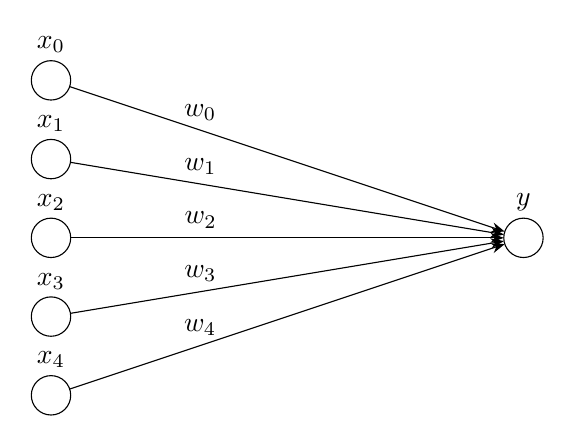
\begin{tikzpicture}
    \draw[->] (0.23717082451262844, 3.9209430584957907) to (5.762829175487371, 2.0790569415042093);
    \draw (0, 4) circle (0.25cm);
    \node at (0, 4.45) { $x_0$ };
    \node[above] at (1.8948683298050513, 3.368377223398316) { $w_0$ };
    \draw[->] (0.24659848095803594, 2.9589002531736606) to (5.753401519041964, 2.0410997468263394);
    \draw (0, 3) circle (0.25cm);
    \node at (0, 3.45) { $x_1$ };
    \node[above] at (1.8986393923832146, 2.683560101269464) { $w_1$ };
    \draw[->] (0.25, 2.0) to (5.75, 2.0);
    \draw (0, 2) circle (0.25cm);
    \node at (0, 2.45) { $x_2$ };
    \node[above] at (1.9, 2.0) { $w_2$ };
    \draw[->] (0.24659848095803594, 1.0410997468263392) to (5.753401519041964, 1.9589002531736608);
    \draw (0, 1) circle (0.25cm);
    \node at (0, 1.45) { $x_3$ };
    \node[above] at (1.8986393923832146, 1.3164398987305357) { $w_3$ };
    \draw[->] (0.23717082451262844, 0.07905694150420949) to (5.762829175487371, 1.9209430584957905);
    \draw (0, 0) circle (0.25cm);
    \node at (0, 0.45) { $x_4$ };
    \node[above] at (1.8948683298050513, 0.6316227766016838) { $w_4$ };
    \draw (6, 2) circle (0.25cm);
    \node at (6, 2.45) { $y$ };
  \end{tikzpicture}
  \end{center}
  In such a graphical representation, the set of $x_i$ nodes are called the \textbf{input layer} (or simply the first layer)
  and the $y$ node is called the \textbf{output layer}. In the above diagram, the output layer 
  consists of one node, but as we will see it can also consist of multiple nodes.

  The output is obtained as a function of the input and weights as below.
  \[
    y = \sum_{i} w_ix_i  
  \] 
  From a statistics perspective, this is actually just a \textbf{linear model}. In statistics, 
  one ``trains'' such a linear model via linear regression on some dataset. If you have 
  taken a statistics course, you might remember that this strategy works on simple 
  examples (e.g., a suspiciously-already-linear weather dataset in a Pearson textbook), 
  but linear models do not generalize and often fail to capture complex behavior.

  As we will see, neural networks are different from linear models since they add properties 
  of hidden layers and nonlinearity.
  
  \section{Hidden Layers}

  Neural networks extend our previous notion of a linear model via \textbf{hidden layers}, which can 
  be defined as one or more layers between the input and output layer. Below, we have 
  a neural network which has one hidden layer. The hidden layer can 
  have a variable number of nodes.

  In this example, each input node $w_i$ connects to each node $h_j$ in the hidden layer 
  via a weight $w_{ij}$. These weights are illustrated by the arrows, although we are 
  choosing to suppress the $w_{ij}$ notation in the diagram below to not over complicate the figure.  
  \begin{center}
    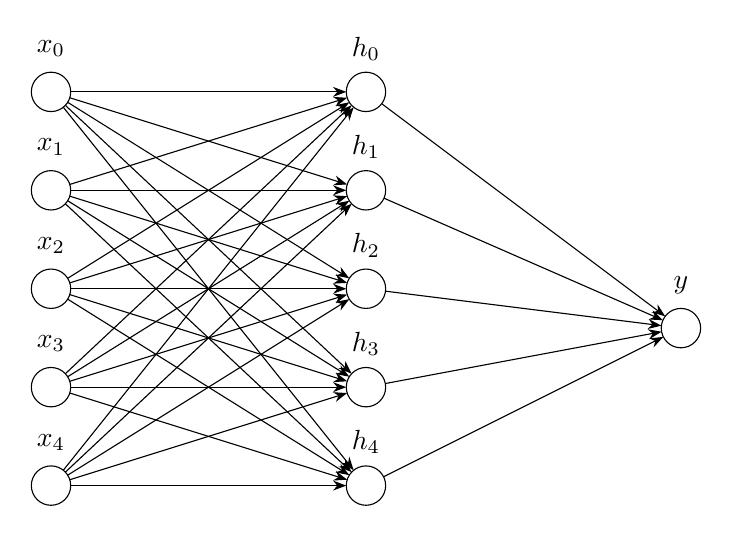
\begin{tikzpicture}
      \draw (0, 5.0) circle (0.25cm);
      \node at (0, 5.55) { $x_0$ };
      \draw (0, 3.75) circle (0.25cm);
      \node at (0, 4.3) { $x_1$ };
      \draw (0, 2.5) circle (0.25cm);
      \node at (0, 3.05) { $x_2$ };
      \draw (0, 1.25) circle (0.25cm);
      \node at (0, 1.8) { $x_3$ };
      \draw (0, 0.0) circle (0.25cm);
      \node at (0, 0.55) { $x_4$ };
      \draw (4, 5.0) circle (0.25cm);
      \node at (4, 5.55) { $h_0$ };
      \draw (4, 3.75) circle (0.25cm);
      \node at (4, 4.3) { $h_1$ };
      \draw (4, 2.5) circle (0.25cm);
      \node at (4, 3.05) { $h_2$ };
      \draw (4, 1.25) circle (0.25cm);
      \node at (4, 1.8) { $h_3$ };
      \draw (4, 0.0) circle (0.25cm);
      \node at (4, 0.55) { $h_4$ };
      \draw (8, 2) circle (0.25cm);
      \node at (8, 2.55) { $y$ };
      \draw[->] (0.25, 5.0) to (3.75, 5.0);
      \draw[->] (0.23861999450875743, 4.925431251716013) to (3.7613800054912425, 3.8245687482839865);
      \draw[->] (0.21199957600127198, 4.867500264999205) to (3.788000423998728, 2.632499735000795);
      \draw[->] (0.1823843010350213, 4.829014717779668) to (3.8176156989649788, 1.4209852822203324);
      \draw[->] (0.15617376188860607, 4.804782797639242) to (3.843826238111394, 0.19521720236075757);
      \draw[->] (0.23861999450875743, 3.8245687482839865) to (3.7613800054912425, 4.925431251716013);
      \draw[->] (0.25, 3.75) to (3.75, 3.75);
      \draw[->] (0.23861999450875743, 3.6754312517160135) to (3.7613800054912425, 2.5745687482839865);
      \draw[->] (0.21199957600127198, 3.617500264999205) to (3.788000423998728, 1.382499735000795);
      \draw[->] (0.1823843010350213, 3.5790147177796676) to (3.8176156989649788, 0.17098528222033244);
      \draw[->] (0.21199957600127198, 2.632499735000795) to (3.788000423998728, 4.867500264999205);
      \draw[->] (0.23861999450875743, 2.5745687482839865) to (3.7613800054912425, 3.6754312517160135);
      \draw[->] (0.25, 2.5) to (3.75, 2.5);
      \draw[->] (0.23861999450875743, 2.4254312517160135) to (3.7613800054912425, 1.3245687482839867);
      \draw[->] (0.21199957600127198, 2.367500264999205) to (3.788000423998728, 0.132499735000795);
      \draw[->] (0.1823843010350213, 1.4209852822203324) to (3.8176156989649788, 4.829014717779668);
      \draw[->] (0.21199957600127198, 1.382499735000795) to (3.788000423998728, 3.617500264999205);
      \draw[->] (0.23861999450875743, 1.3245687482839867) to (3.7613800054912425, 2.4254312517160135);
      \draw[->] (0.25, 1.25) to (3.75, 1.25);
      \draw[->] (0.23861999450875743, 1.1754312517160133) to (3.7613800054912425, 0.07456874828398671);
      \draw[->] (0.15617376188860607, 0.19521720236075757) to (3.843826238111394, 4.804782797639242);
      \draw[->] (0.1823843010350213, 0.17098528222033244) to (3.8176156989649788, 3.5790147177796676);
      \draw[->] (0.21199957600127198, 0.132499735000795) to (3.788000423998728, 2.367500264999205);
      \draw[->] (0.23861999450875743, 0.07456874828398671) to (3.7613800054912425, 1.1754312517160133);
      \draw[->] (0.25, -1.5308084989341915e-17) to (3.75, 1.5308084989341915e-17);
      \draw[->] (4.2, 4.85) to (7.8, 2.15);
      \draw[->] (4.229039333725547, 3.649795291495073) to (7.770960666274453, 2.100204708504927);
      \draw[->] (4.248069469178417, 2.4689913163526978) to (7.751930530821583, 2.0310086836473022);
      \draw[->] (4.245718046733581, 1.2960721337625463) to (7.754281953266419, 1.9539278662374537);
      \draw[->] (4.223606797749979, 0.11180339887498945) to (7.776393202250021, 1.8881966011250106);
    \end{tikzpicture}
  \end{center}
  The calculation of a hidden layer is simply 
  \[
      h_j = \sum_{i}w_{ij}x_i
  \]  
  Intuitively, this means that each input value $x_i$ makes a weighted contribution of $w_{ij}$ 
  to the value $h_j$. Something to observe at this point is that we can summarize the entire hidden layer 
  calculation as a matrix equation:
  \begin{align}
    \vec{h}=
    \begin{bmatrix}
      h_{1} \\
      h_{2} \\
      h_{3} \\
      h_{4} \\
      h_{5}
    \end{bmatrix}
    = \begin{bmatrix}
      \sum_{i}w_{i1}x_i \\
      \sum_{i}w_{i2}x_i \\
      \sum_{i}w_{i3}x_i \\
      \sum_{i}w_{i4}x_i \\
      \sum_{i}w_{i5}x_i \\
    \end{bmatrix}
    = \begin{bmatrix}
      w_{11} & w_{12} & w_{13} & w_{14} & w_{15} \\
      w_{21} & w_{22} & w_{23} & w_{24} & w_{25} \\
      w_{31} & w_{32} & w_{33} & w_{34} & w_{35} \\
      w_{41} & w_{42} & w_{43} & w_{44} & w_{45} \\
      w_{51} & w_{52} & w_{53} & w_{54} & w_{55} \\
    \end{bmatrix}
    \cdot
    \begin{bmatrix}
      x_{1} \\
      x_{2} \\
      x_{3} \\
      x_{4} \\
      x_{5}
    \end{bmatrix}
    = 
    W\vec{x}
  \end{align}
  This suggest the concept of a \textbf{weight matrix} $W$, which is the key to calculating the 
  hidden layer $\vec{h}$ from the input $\vec{x}$.

  As we can see, between each layer we have a matrix of weights. We can denote $U$ as the matrix of 
  the weights between the output layer and the hidden layer, so that 
  $y = U\vec{h}$. However, note that 
  \[
      y = U\vec{h} = UW\vec{x} = W'\vec{x}
  \]
  where $W' = UW$. This reduces our above network, with three layers, to a boring network, with two layers (similar to the one 
  we started with), just with a different weight matrix $W'$. The reason is because our network is linear, which means 
  no matter how many layers we add it will always reduce to the same boring network we started with. 
  Thus in order to get something interesting with hidden layers we need to add some nonlinearity.
  
  \section{Nonlinearity}
  Neural networks achieve our desired property of nonlinearity via usage of \textbf{activation fuctions}.
  A few common examples of such functions are the sigmoid, tanh or RELU functions, and the choice of an activation 
  function depends on what one is trying to achieve with a neural network. 

  The sigmoid function is given by
  \[
      \sigma(x) = \frac{1}{1 + e^{-x}}
  \]
  The graph of the sigmoid function is given below.
  \begin{center}
    \begin{tikzpicture}
      \begin{scope}
    \draw[Gray!30, ->] (-4, 0) to (4, 0);
    \draw[Gray!30, ->] (0, 0) to (0, 5.0);
    \node[below] at (4, 0) { $x$ };
    \node[left] at (0, 5.0) { $y$ };
  \end{scope}
  
      \draw[dashed] (-3.5, 4.5) to (4.5, 4.5);
      \draw[fill] (0, 4.5) circle (0.01cm);
      \node[left] at (-3.5, 4.5) { $y=1$ };
      \draw[ProcessBlue] plot coordinates {(-4.5, 0.005262796192749818) (-4.454773869346734, 0.005631746396210898) (-4.409547738693467, 0.006026527305014147) (-4.364321608040201, 0.006448942330119109) (-4.319095477386934, 0.006900920060491525) (-4.273869346733669, 0.0073845228460029805) (-4.228643216080402, 0.007901955953416093) (-4.183417085427136, 0.008455577331464884) (-4.138190954773869, 0.009047908022967094) (-4.092964824120603, 0.009681643263881561) (-4.047738693467337, 0.01035966431124376) (-4.00251256281407, 0.011085051043962974) (-3.9572864321608043, 0.011861095382535868) (-3.9120603015075375, 0.01269131557580394) (-3.866834170854271, 0.013579471404940771) (-3.821608040201005, 0.014529580356873897) (-3.776381909547739, 0.015545934821298967) (-3.7311557788944727, 0.01663312036729784) (-3.685929648241206, 0.017796035157289784) (-3.64070351758794, 0.019039910557579216) (-3.5954773869346734, 0.020370333006064664) (-3.550251256281407, 0.02179326719867715) (-3.505025125628141, 0.02331508065675532) (-3.459798994974874, 0.024942569737754265) (-3.414572864321608, 0.026682987151332882) (-3.369346733668342, 0.0285440710418642) (-3.324120603015076, 0.030534075696637793) (-3.2788944723618094, 0.032661803936339655) (-3.2336683417085426, 0.03493664124063683) (-3.1884422110552766, 0.037368591656690056) (-3.14321608040201, 0.03996831553195919) (-3.0979899497487438, 0.04274716910453138) (-3.052763819095478, 0.0457172459741365) (-3.007537688442211, 0.04889142046473615) (-2.9623115577889445, 0.05228339287476804) (-2.9170854271356785, 0.05590773659345733) (-2.871859296482412, 0.059779947040685594) (-2.8266331658291457, 0.06391649236333043) (-2.7814070351758797, 0.06833486579230547) (-2.7361809045226133, 0.07305363953125817) (-2.690954773869347, 0.07809252000951472) (-2.6457286432160805, 0.0834724042878502) (-2.600502512562814, 0.08921543735544614) (-2.555276381909548, 0.09534506999939227) (-2.5100502512562812, 0.10188611686370903) (-2.4648241206030153, 0.10886481424252653) (-2.419597989949749, 0.11630887707120185) (-2.3743718592964824, 0.12424755448927133) (-2.329145728643216, 0.13271168324978544) (-2.28391959798995, 0.1417337381404277) (-2.2386934673366836, 0.15134787846268502) (-2.193467336683417, 0.16158998948623748) (-2.148241206030151, 0.1724977176569227) (-2.1030150753768844, 0.18411049818868822) (-2.057788944723618, 0.19646957351385033) (-2.012562814070352, 0.20961800090317478) (-1.9673366834170856, 0.2236006473998081) (-1.9221105527638191, 0.23846417004160023) (-1.8768844221105527, 0.2542569791783549) (-1.8316582914572865, 0.2710291825283369) (-1.7864321608040203, 0.2888325074673447) (-1.741206030150754, 0.30772019891019453) (-1.6959798994974875, 0.32774689003619695) (-1.650753768844221, 0.3489684430359182) (-1.605527638190955, 0.37144175702627613) (-1.5603015075376887, 0.39522454030606535) (-1.5150753768844223, 0.420375044216673) (-1.4698492462311556, 0.4469517560462967) (-1.4246231155778895, 0.4750130486842121) (-1.3793969849246233, 0.5046167851086218) (-1.334170854271357, 0.5358198762909183) (-1.2889447236180909, 0.5686777917334077) (-1.243718592964824, 0.603244022637125) (-1.1984924623115578, 0.6395694986289344) (-1.1532663316582916, 0.677701960065948) (-1.1080402010050254, 0.717685289178302) (-1.0628140703517592, 0.7595588046996393) (-1.0175879396984924, 0.803356526151213) (-0.9723618090452262, 0.8491064155640977) (-0.92713567839196, 0.8968296061080361) (-0.8819095477386938, 0.946539628797629) (-0.8366834170854276, 0.9982416501087256) (-0.7914572864321607, 1.0519317348915715) (-0.7462311557788945, 1.1075961503353762) (-0.7010050251256283, 1.1652107278379473) (-0.6557788944723622, 1.224740300377231) (-0.610552763819096, 1.2861382332838076) (-0.5653266331658291, 1.3493460660955867) (-0.5201005025125629, 1.414293282371383) (-0.4748743718592967, 1.4808972229002506) (-0.4296482412060305, 1.549063155643788) (-0.3844221105527643, 1.618684512994169) (-0.33919597989949746, 1.6896433035594725) (-0.29396984924623126, 1.7618107017739604) (-0.24874371859296507, 1.835047814283836) (-0.20351758793969887, 1.9092066174213018) (-0.158291457286432, 1.9841310553222182) (-0.11306532663316582, 2.0596582835558777) (-0.06783919597989962, 2.135620038720231) (-0.02261306532663343, 2.2118441105114752) (0.022613065326632764, 2.288155889488524) (0.06783919597989962, 2.364379961279769) (0.11306532663316582, 2.4403417164441223) (0.158291457286432, 2.515868944677782) (0.2035175879396982, 2.5907933825786973) (0.2487437185929644, 2.6649521857161633) (0.29396984924623126, 2.738189298226039) (0.33919597989949746, 2.8103566964405275) (0.38442211055276365, 2.88131548700583) (0.42964824120602985, 2.9509368443562107) (0.47487437185929604, 3.0191027770997483) (0.5201005025125629, 3.085706717628617) (0.5653266331658291, 3.1506539339044135) (0.6105527638190953, 3.2138617667161915) (0.6557788944723615, 3.275259699622768) (0.7010050251256277, 3.334789272162052) (0.7462311557788945, 3.3924038496646243) (0.7914572864321607, 3.4480682651084287) (0.8366834170854269, 3.5017583498912734) (0.8819095477386931, 3.5534603712023705) (0.9271356783919593, 3.603170393891963) (0.9723618090452262, 3.6508935844359023) (1.0175879396984924, 3.6966434738487868) (1.0628140703517586, 3.74044119530036) (1.1080402010050248, 3.782314710821697) (1.153266331658291, 3.822298039934051) (1.1984924623115578, 3.860430501371066) (1.243718592964824, 3.8967559773628744) (1.2889447236180902, 3.931322208266592) (1.3341708542713564, 3.964180123709081) (1.3793969849246226, 3.9953832148913775) (1.4246231155778895, 4.024986951315788) (1.4698492462311556, 4.053048243953704) (1.5150753768844218, 4.079624955783327) (1.5603015075376887, 4.1047754596939345) (1.6055276381909542, 4.128558242973723) (1.650753768844221, 4.1510315569640825) (1.6959798994974866, 4.172253109963803) (1.7412060301507535, 4.192279801089805) (1.7864321608040203, 4.211167492532655) (1.8316582914572859, 4.228970817471663) (1.8768844221105527, 4.245743020821645) (1.9221105527638183, 4.261535829958399) (1.9673366834170851, 4.276399352600191) (2.012562814070352, 4.290381999096825) (2.0577889447236175, 4.30353042648615) (2.1030150753768844, 4.315889501811312) (2.14824120603015, 4.327502282343077) (2.1934673366834168, 4.338410010513762) (2.2386934673366836, 4.348652121537315) (2.283919597989949, 4.358266261859572) (2.329145728643216, 4.367288316750215) (2.3743718592964815, 4.375752445510728) (2.4195979899497484, 4.3836911229287985) (2.4648241206030153, 4.391135185757473) (2.510050251256281, 4.398113883136291) (2.5552763819095476, 4.404654930000608) (2.600502512562813, 4.410784562644554) (2.64572864321608, 4.41652759571215) (2.690954773869347, 4.421907479990486) (2.7361809045226124, 4.426946360468742) (2.7814070351758793, 4.4316651342076945) (2.826633165829145, 4.4360835076366705) (2.8718592964824117, 4.440220052959314) (2.9170854271356785, 4.444092263406542) (2.962311557788944, 4.447716607125232) (3.007537688442211, 4.451108579535264) (3.0527638190954764, 4.454282754025863) (3.0979899497487433, 4.457252830895468) (3.14321608040201, 4.46003168446804) (3.1884422110552757, 4.462631408343309) (3.2336683417085426, 4.465063358759363) (3.278894472361808, 4.46733819606366) (3.324120603015075, 4.469465924303362) (3.369346733668342, 4.471455928958136) (3.4145728643216073, 4.473317012848668) (3.459798994974874, 4.475057430262245) (3.5050251256281397, 4.476684919343245) (3.5502512562814066, 4.478206732801323) (3.5954773869346734, 4.479629666993935) (3.640703517587939, 4.480960089442421) (3.685929648241206, 4.48220396484271) (3.7311557788944714, 4.483366879632702) (3.7763819095477382, 4.484454065178701) (3.821608040201005, 4.485470419643126) (3.8668341708542706, 4.486420528595058) (3.9120603015075375, 4.487308684424196) (3.957286432160803, 4.488138904617464) (4.00251256281407, 4.488914948956037) (4.047738693467337, 4.4896403356887555) (4.092964824120602, 4.490318356736118) (4.138190954773869, 4.490952091977033) (4.183417085427136, 4.491544422668535) (4.2286432160804015, 4.492098044046584) (4.273869346733669, 4.492615477153997) (4.319095477386934, 4.493099079939508) (4.364321608040201, 4.493551057669881) (4.409547738693467, 4.493973472694987) (4.454773869346733, 4.494368253603789) (4.5, 4.49473720380725) };
  \end{tikzpicture}
  \end{center}
  


  Using our previous network, we can modify 
  

  
  \section{Backpropagation}








\end{document}